% !TEX root =  master.tex
\chapter{Evaluation}\label{chapter:evaluation}


\section{Evaluation of ResNeXt} \label{chapter:eval_resnext}
\sectionauthor{Written by Tobias Richstein}

The training of the ResNeXt went very well. As can be seen in figure \vref{fig:resnext_eval} the relevant metrics of Accuracy, F1 score, Recall and precision keep going up during training. Now it is important to stress two things: First, we are not actually too interested in getting perfect results from this model in terms of classifying the 14 illnesses from the NIH dataset (from section \vref{data:nih}) and second, the number of samples is heavily unbalanced and most images have no findings at all. Especially the second fact explains the rather low recall score (ratio of true positive predictions in a class to all observations of that class) and the resulting low F1 score.

\begin{figure*}[h]
	\centering
	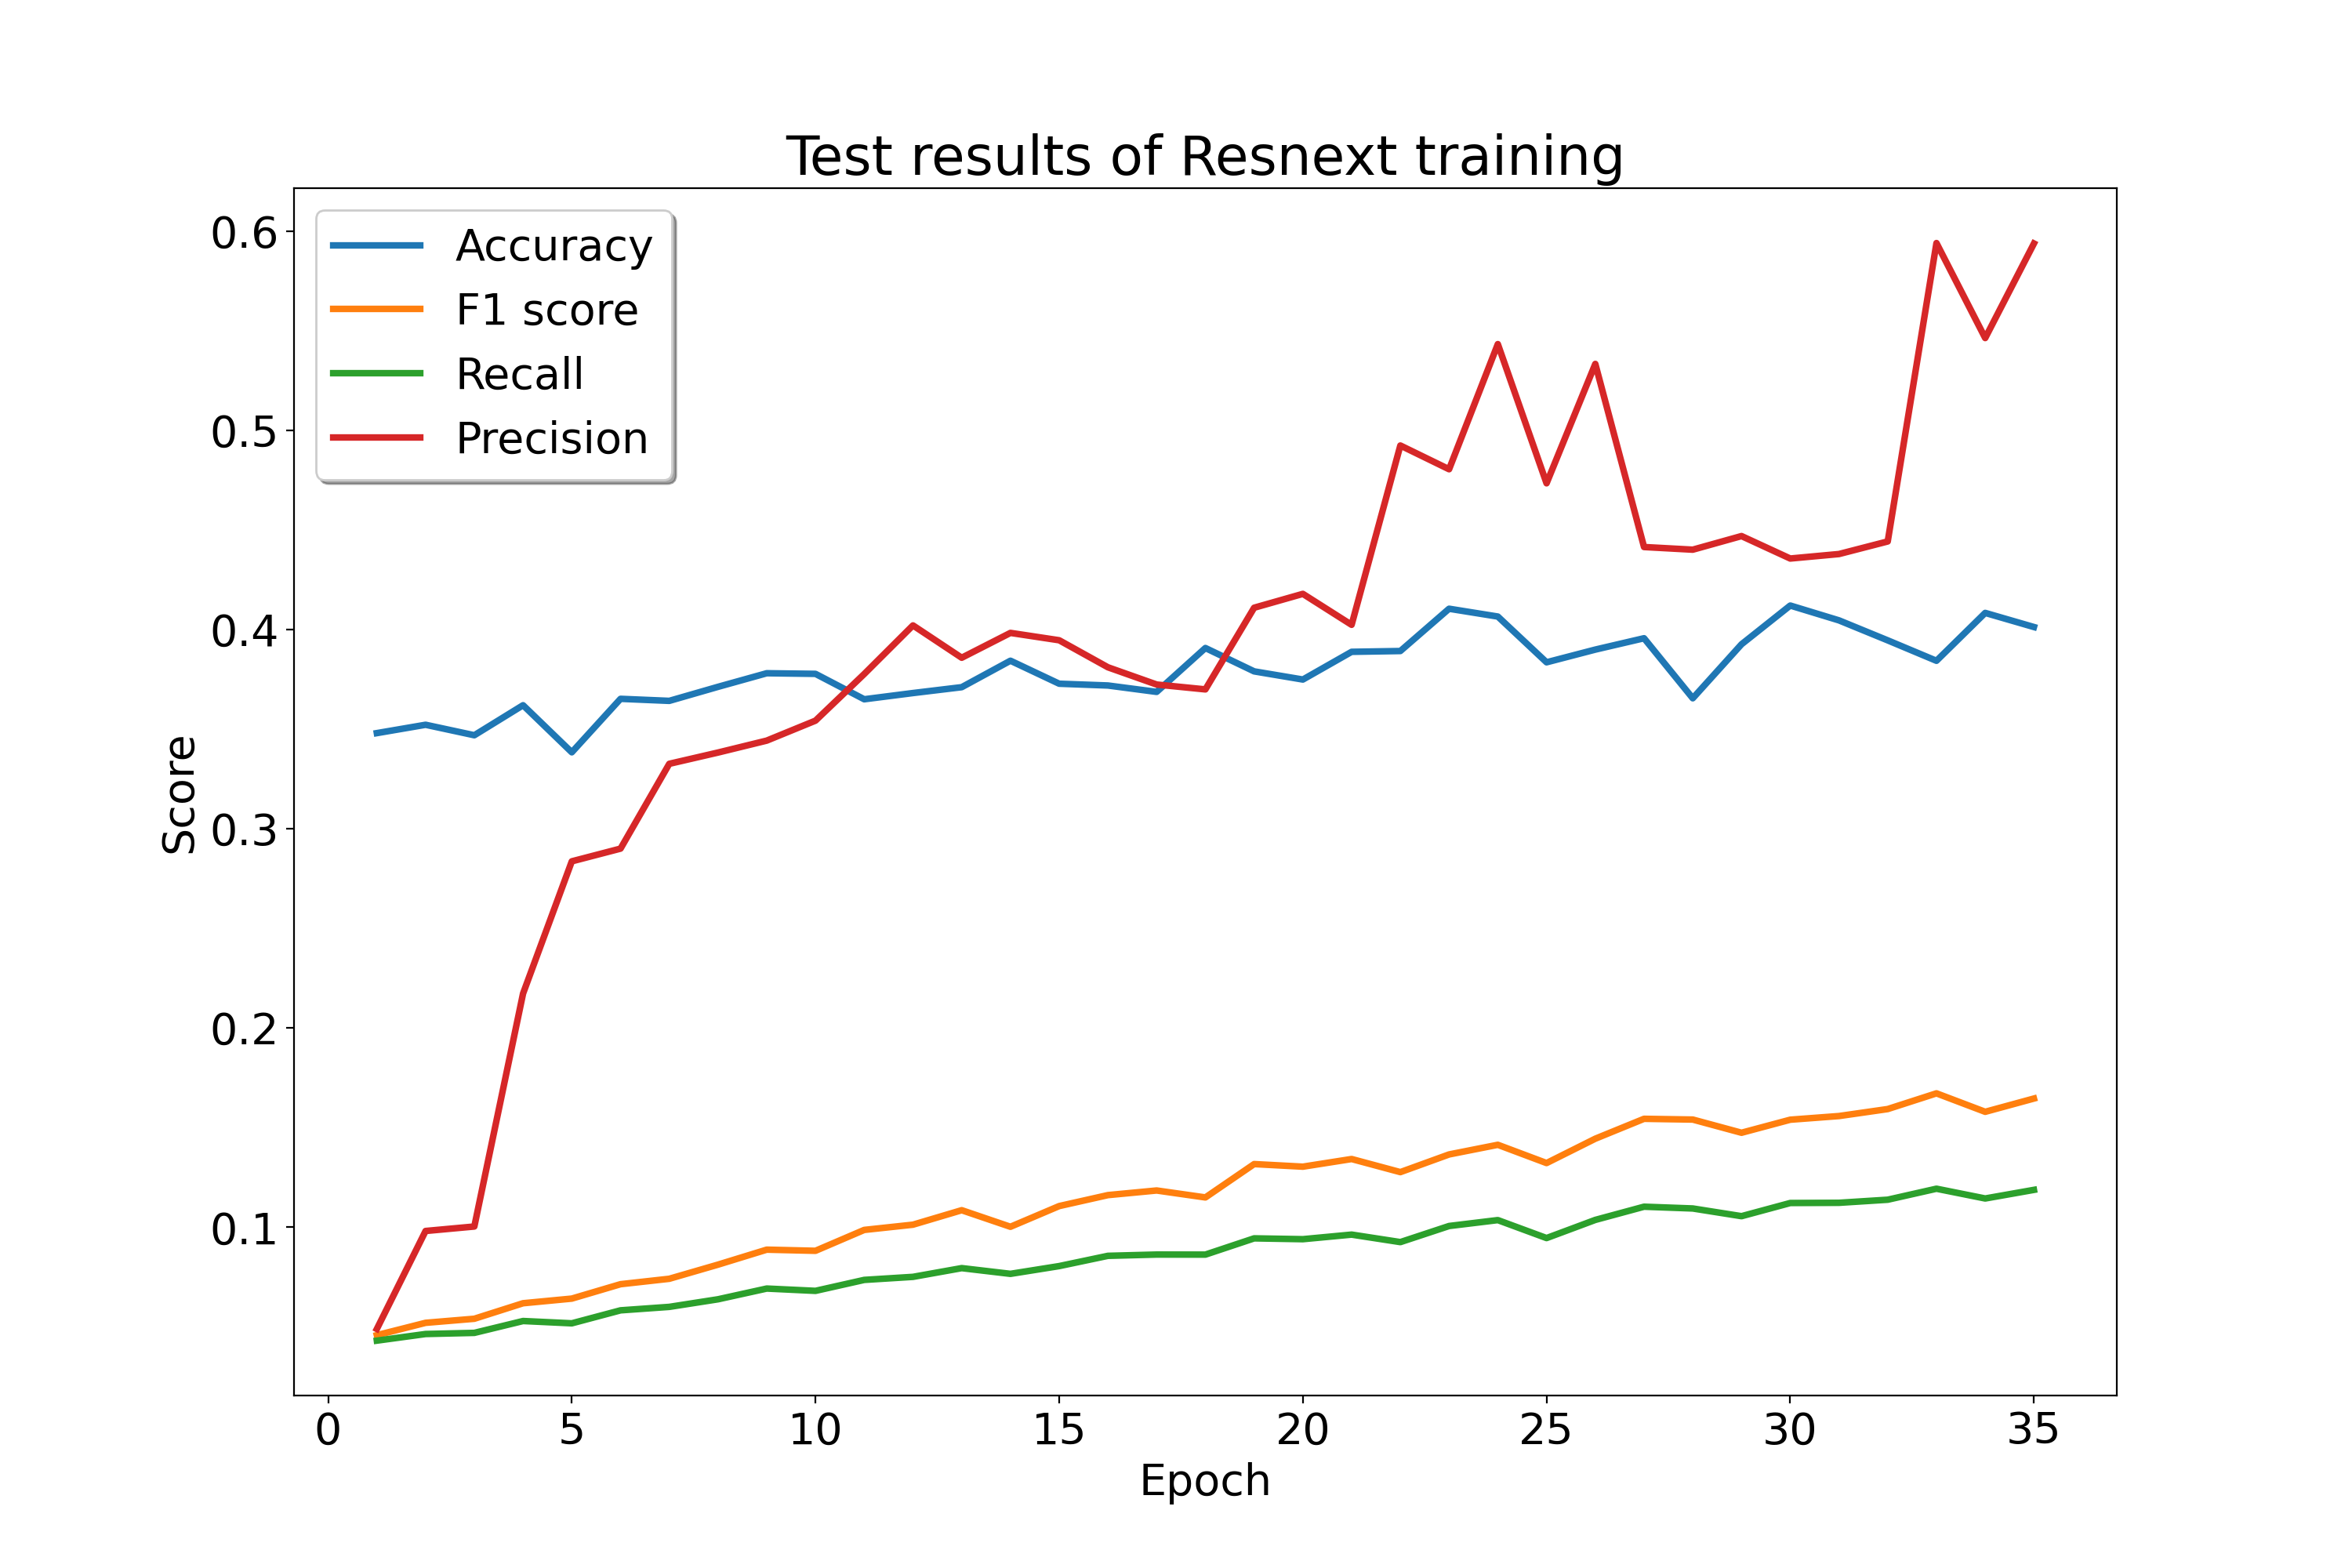
\includegraphics[width=.8\linewidth]{img/test_results_backbone_rcnn_35.png}
	\caption{ResNeXt model metrics during training}
	\label{fig:resnext_eval}
\end{figure*}

In a more refined setup we could have modified the dataloader to for example over-sample all underrepresented or on the other hand under-sample some of the dominant illness labels found in the dataset to balance the training a little more. Since again we are not really interested in the actual classification but more in the feature vectors that we can use as the Faster R-CNN backbone, we are satisfied with a final Precision of $0.59$, Recall of $0.12$, Accuracy of $0.40$ and F1 score of $0.16$. We could also certainly have trained the model further as no dramatic overfit seems to have occurred yet but as will be shown in the next section, the overall results for which we need the backbone are quite satisfactory.

\section{Evaluation of COVID-19 detection}\label{chapter:eval_rcnn_yolo}
\sectionauthor{Written by Julian Seibel}

To evaluate our COVID-19 detection capabilities, we identified two major steps that include the evaluation of the prediction quality for both the detection models, namely Faster \ac{R-CNN} and \ac{YOLO} and the evaluation of our ensemble approach, where we applied the method described previously in \ref{section:combining_detections} to come up with a final prediction considering both model outputs. 

There are multiple metrics possible for measuring the quality of an object detection model. However, we decided to utilize the widely used \acf{mAP} as our crucial performance evaluation metric since many of the contributions in the field of object detection adapted the metric making it the de-facto standard in many open object detection challenges like Pascal VOC \autocite{everingham2010pascal} or COCO \autocite{coco}. The \ac{mAP} considers both, the quality of the class as well as the bounding box prediction. Regarding the latter, the \ac{IoU} between ground truth and prediction is used to measure the placement quality by defining a threshold $t$ which determines if a predicted box will be handled as true positive (\ac{IoU} $> t$) or as false positive (\ac{IoU} $< t$)\footnote{Since it is not necessary to count true negatives as there should just be no box, those values will be excluded also in the computation of recall and precision later on.}. There are various values for $t$ conceivable depending also on the requirements the model needs to fulfill. In general the threshold used is denoted as \ac{mAP}@$t$. In our example we mainly focused on the \ac{mAP}@$.50$ score. Hence, a predicted bounding box will be counted as a true positive if the \ac{IoU} value indicates a 50\% coverage of the ground truth. There are different ways to calculate the final \ac{mAP} score, for example in \autocite{padilla2020survey} the authors propose to use an all-point interpolation method to smooth the precision-recall curve to calculate the final average precision. Since our work only considers one class bounding box prediction (\enquote{opacity}), the \ac{mAP} is reduced to just the average precision (AP).

First, we consider both the models and compare them in terms of our selected metrics in our validation phase that is performed after each training epoch.
For the \ac{YOLO} model, figure \ref{fig:yolo_pretraining_results} shows the validation metrics during pre-training on the \ac{RSNA} data. The graph shows that during the first epochs of the pre-training the metric values increase but then kind of flatten out achieving almost $\approx60\%$ in \ac{mAP}@$.50$. Similar to the ResNeXt backbone model, we are not particularly interested in achieving state-of-the-art scores during pre-training, rather that we experience a continuous learning for \enquote{introducing} the model and its weights to the problem domain.

\begin{figure*}[h!]
	\begin{minipage}[b]{.5\linewidth} % [b] => Ausrichtung an \caption
		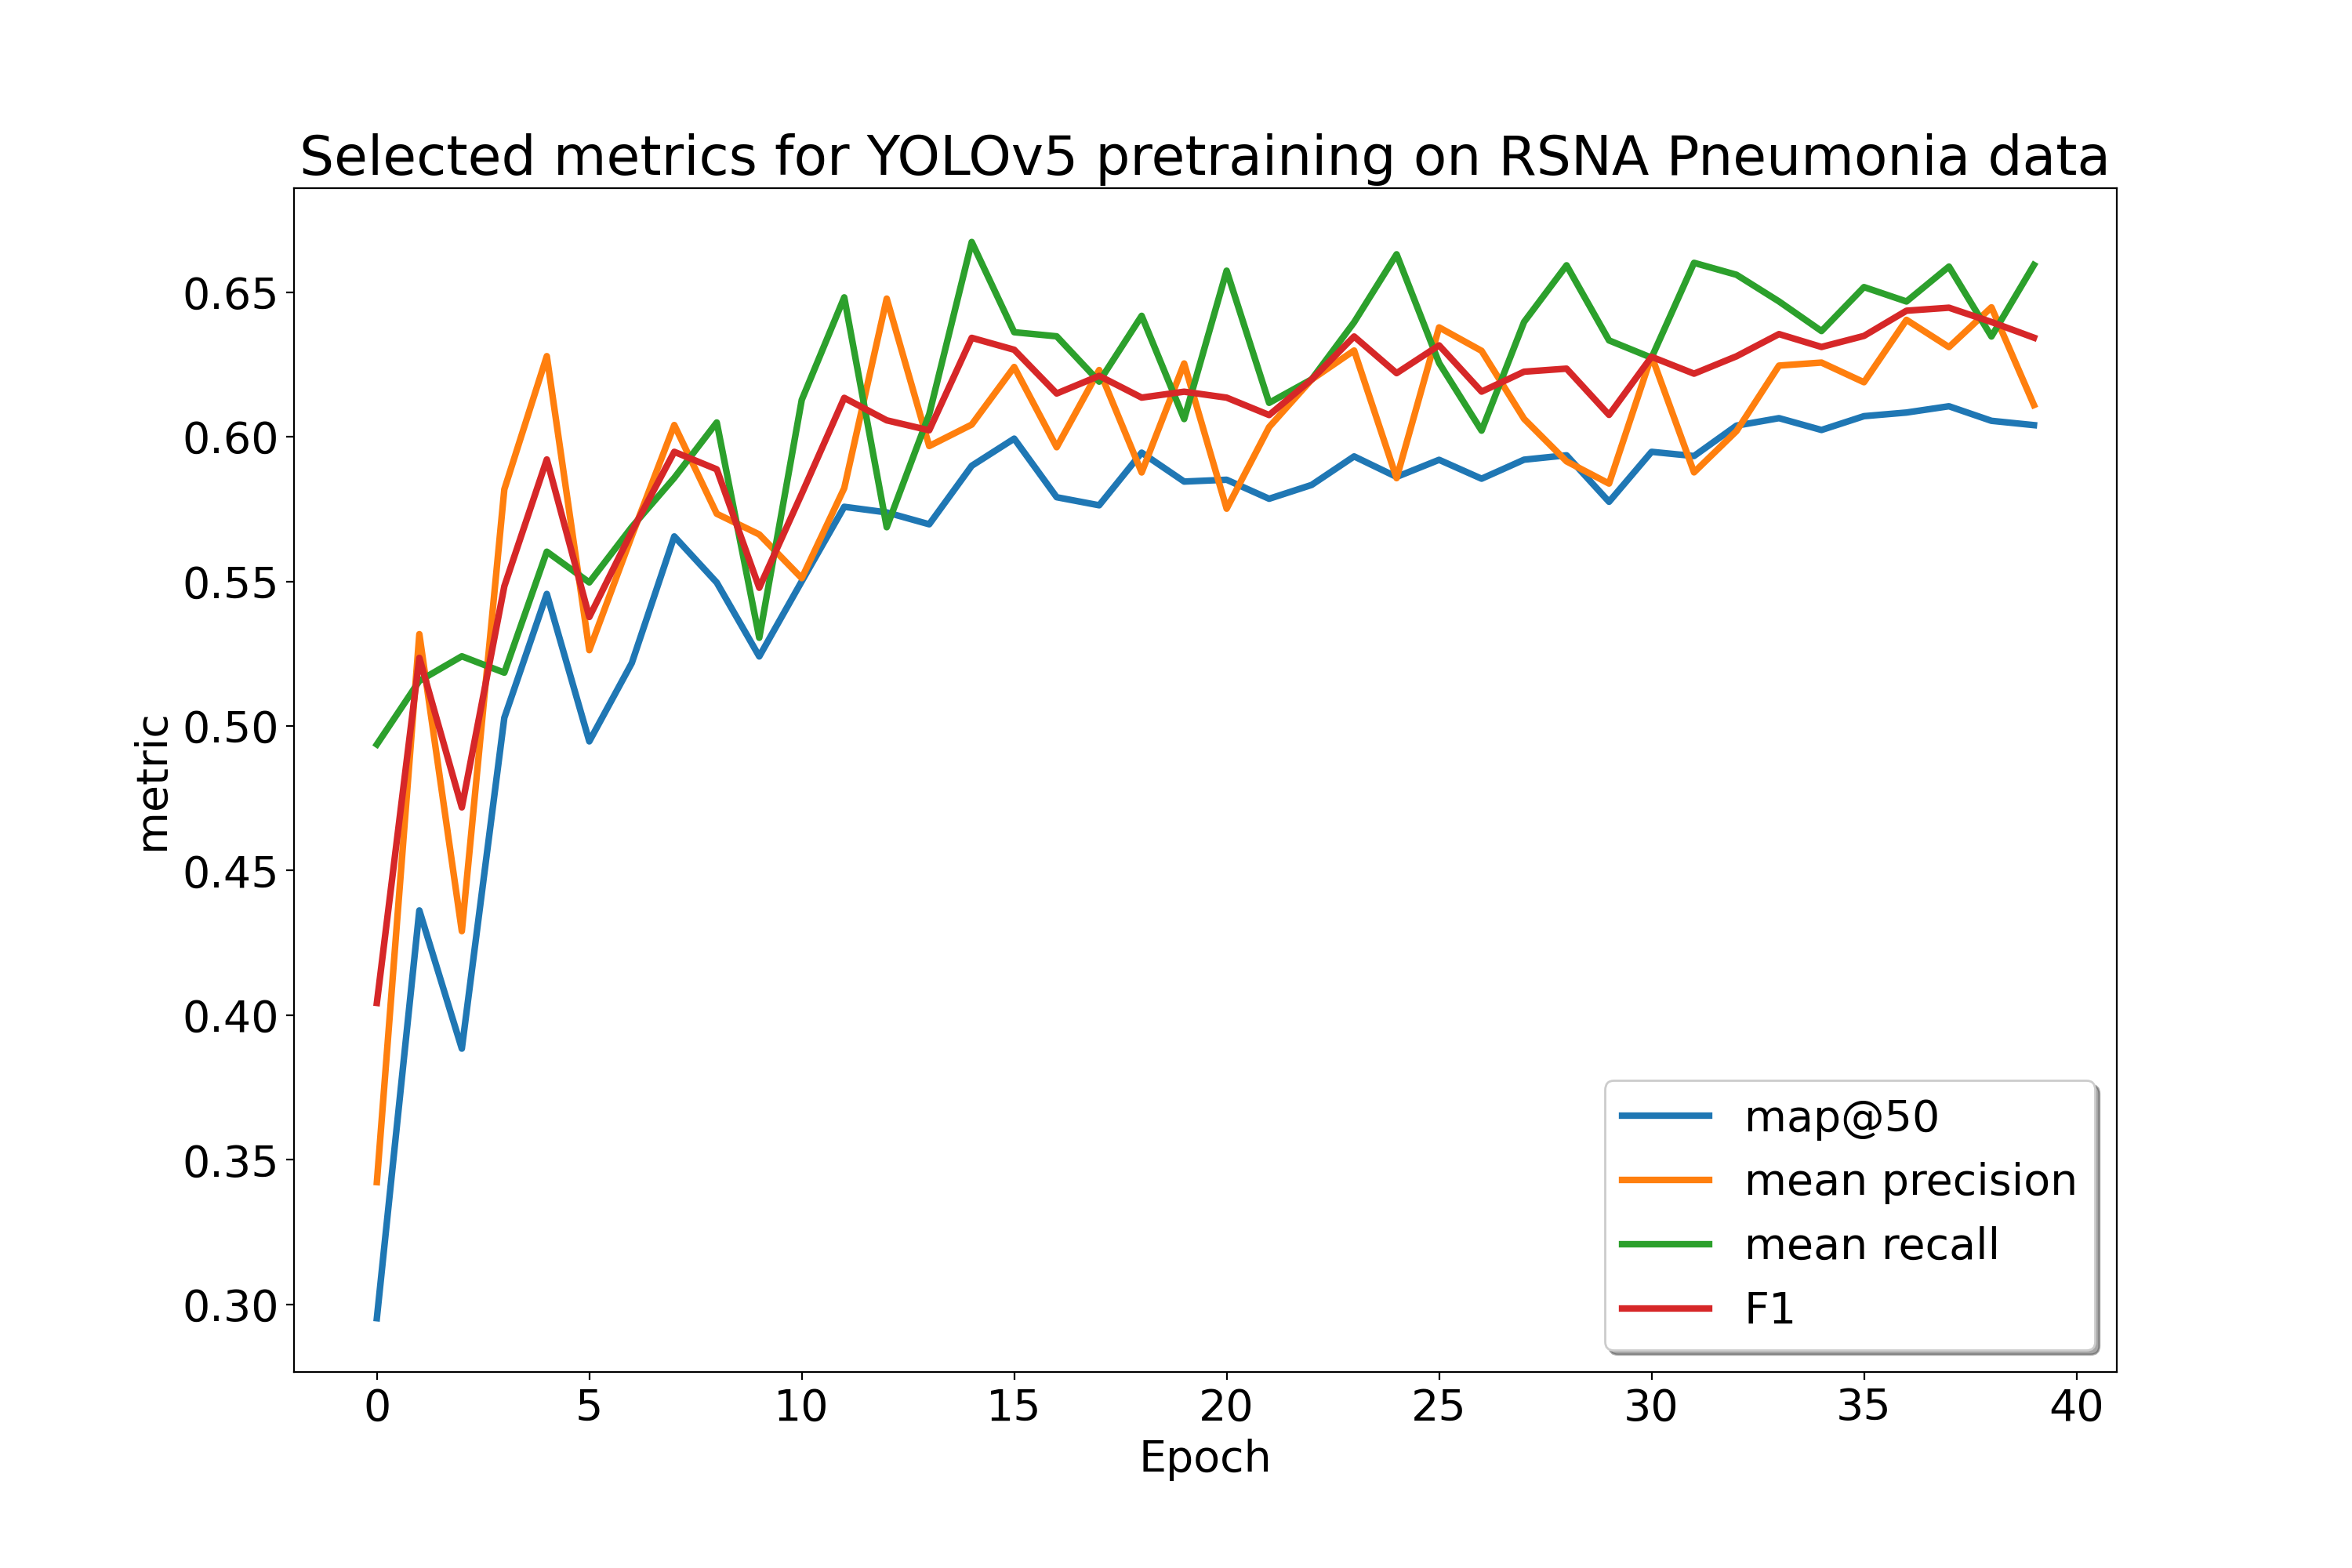
\includegraphics[width=\linewidth]{img/metrics_giou_pretrained_yolo_40.png}
		\caption{Validation results for the \ac{YOLO} pretraining.}
		\label{fig:yolo_pretraining_results}
	\end{minipage}
	\begin{minipage}[b]{.5\linewidth} % [b] => Ausrichtung an \caption
		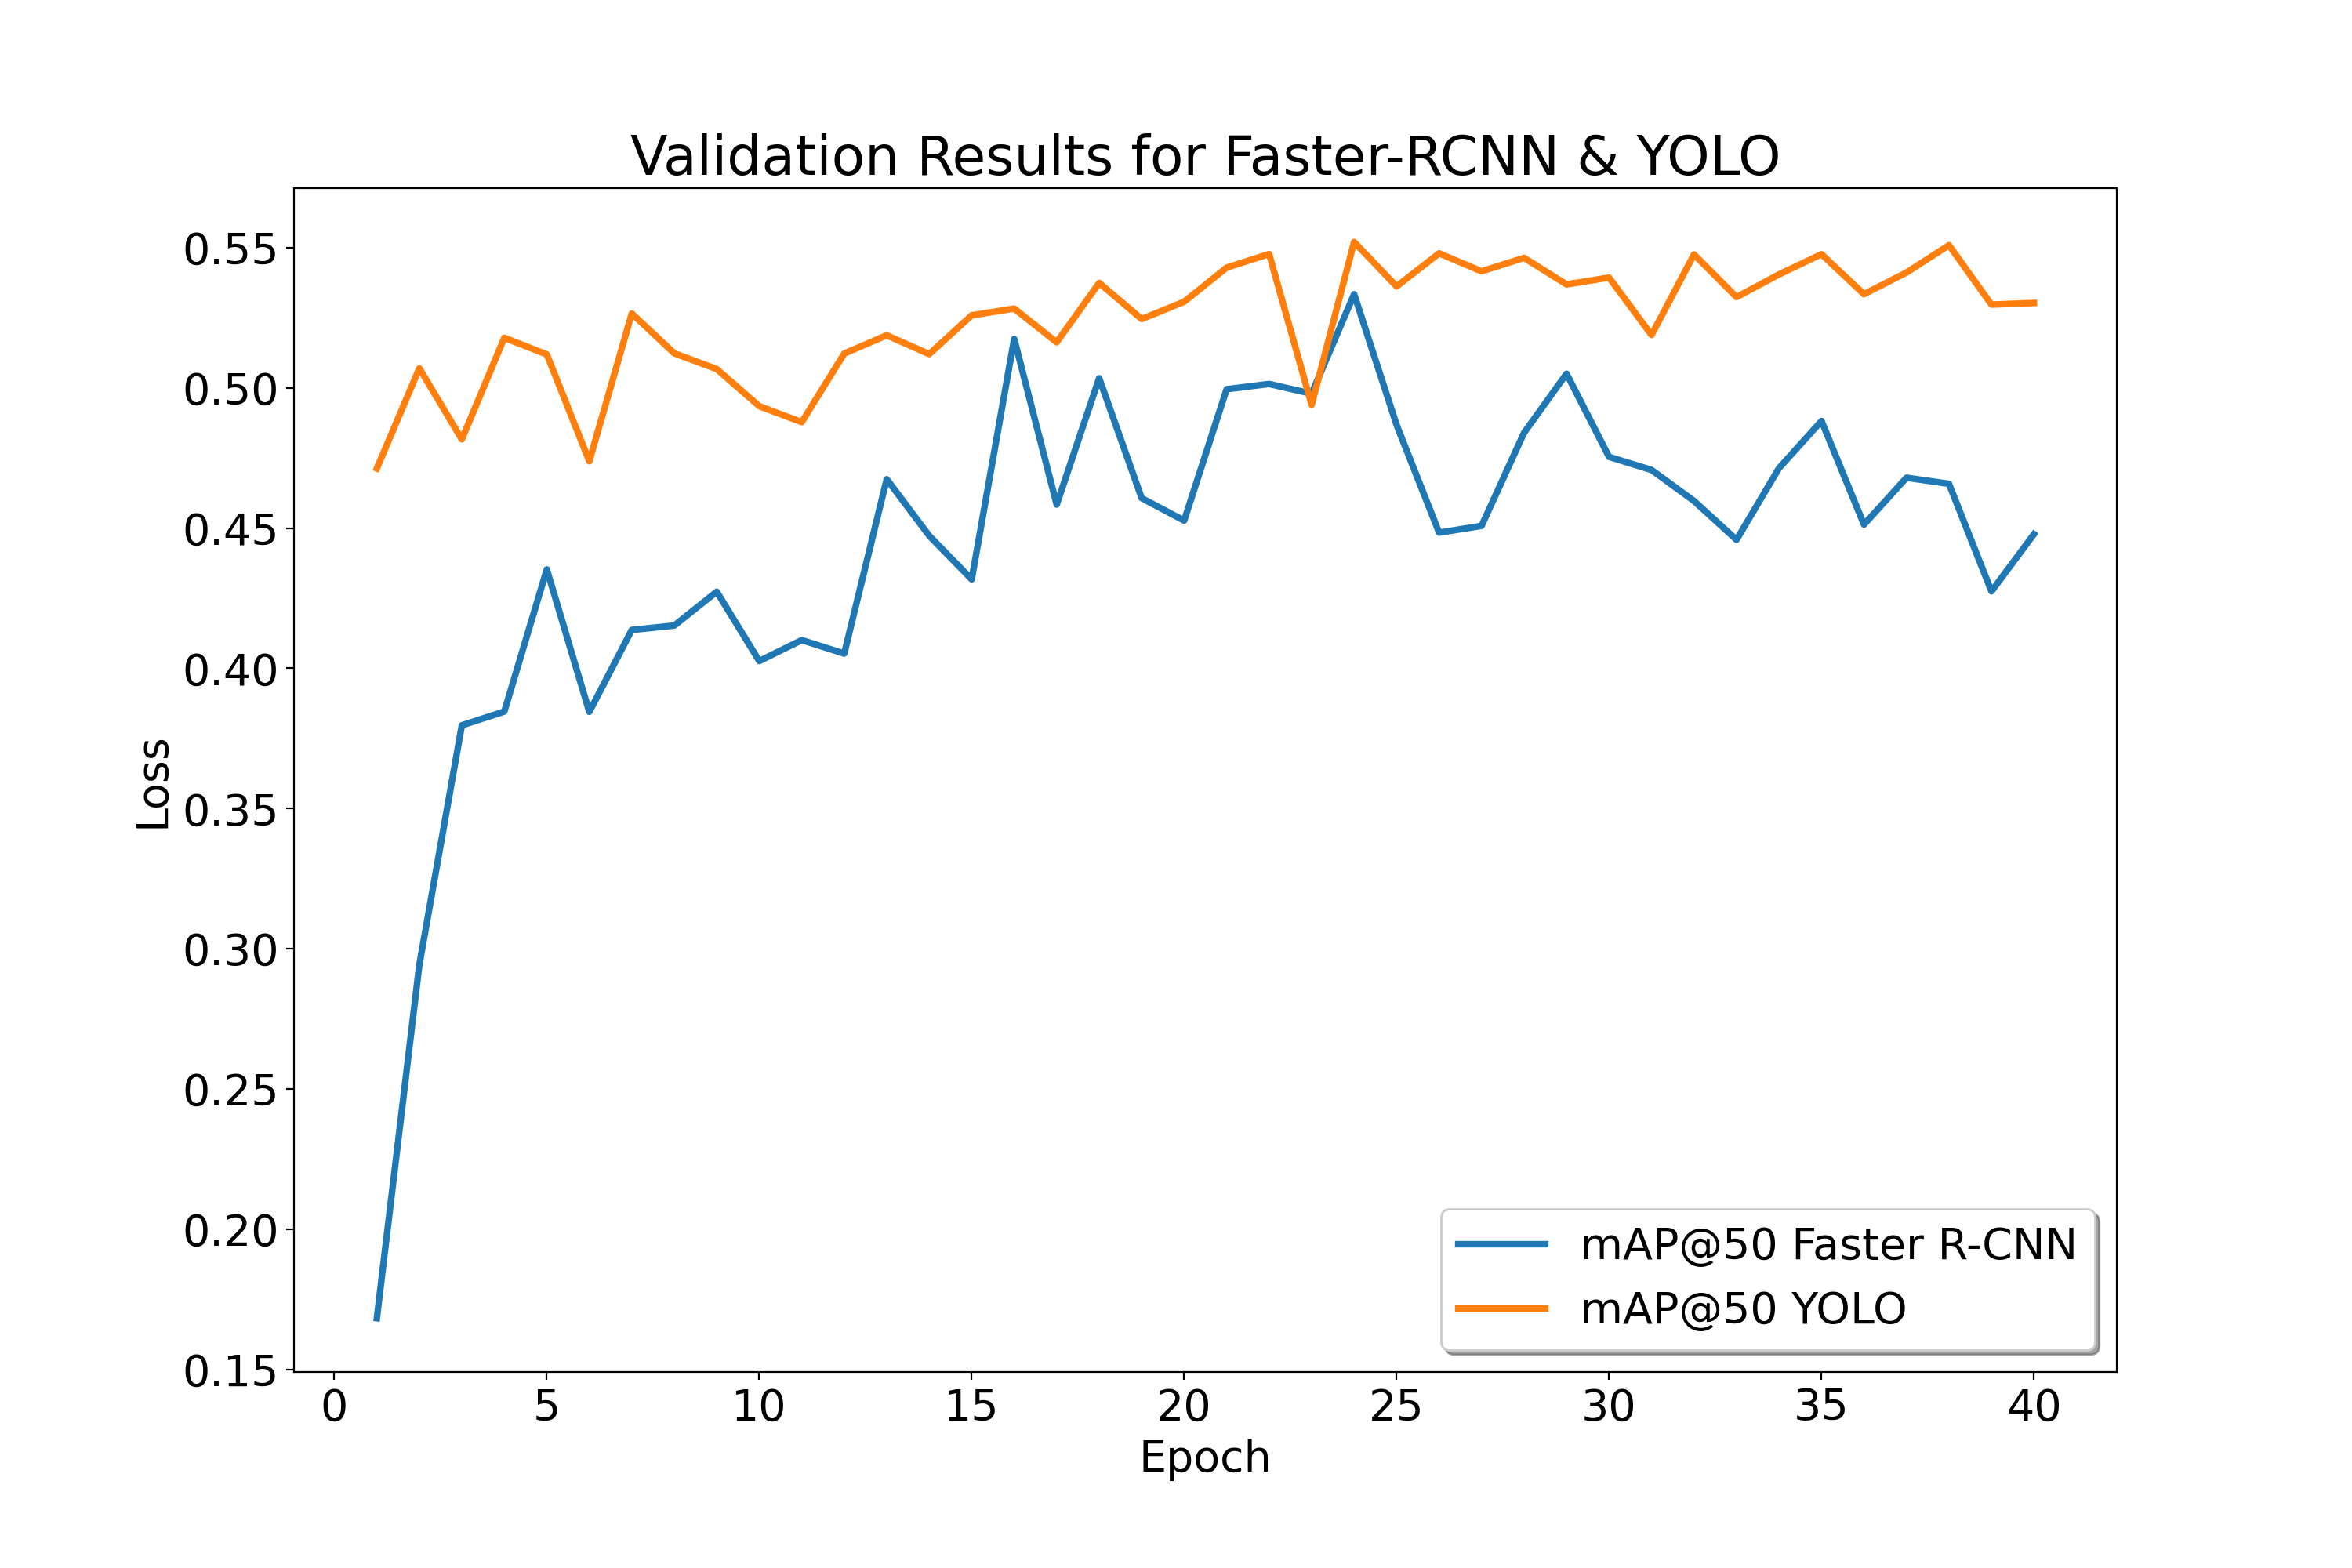
\includegraphics[width=\linewidth]{img/eval_results_ap_only_fasterrcnn_yolo.png}
		\caption{Validation results on the SIIM COVID-19 data.}
		\label{fig:yolo_frcnn_results}
	\end{minipage}
\end{figure*}

The final validation results during training for both detection models on the COVID-19 dataset can be found in \ref{fig:yolo_frcnn_results}. The figure shows that we only see a slow increase in \ac{mAP}@$.50$ for the \ac{YOLO} model which is mainly caused by the pre-training. In contrast, the Faster \ac{R-CNN} model shows a similar pattern like the \ac{YOLO} in pre-training where with an increasing number of epochs the metric values flatten out after a heavy increase in the first epochs. In general, we could observe that the \ac{YOLO} model shows better results with an \ac{mAP}@$.50$ of $\approx 55\%$, whereas the Faster \ac{R-CNN} reaches $\approx 53\%$ in its best epoch. As already indicated in the training sections, we could observe a slight overfit of the model leading to a decreasing score again. This phenomenon might be caused by the limited data available or too long training. Due to time constraints we did not analyze this behavior in more detail and leave this open for further research, including hyper-parameter tuning and cross-validation methods.
However, we chose the best observed models for our final implementation of the COVID-19 detection. In more detail we used the \ac{YOLO} model checkpoint at epoch 26 and the Faster \ac{R-CNN} model checkpoint at epoch 23.

Finally, table \ref{table:final_results} shows extended evaluation results of the models including also the ensemble performance on a held-out set consisting of 859 examples. 
\begin{table}[h]
	\begin{tabular}{l|l|l|l}
		&    Faster R-CNN          &         YOLO             &  Ensemble \\ \hline
		mAP@.50			& \multicolumn{1}{l|}{0.409} & \multicolumn{1}{l|}{0.345} & \textbf{0.451}  \\
		F1-score		& \multicolumn{1}{l|}{0.547} & \multicolumn{1}{l|}{0.477} & \textbf{0.560} \\
		mean Recall		& \multicolumn{1}{l|}{0.503} & \multicolumn{1}{l|}{0.450} & \textbf{0.530} \\
		mean Precision	& \multicolumn{1}{l|}{\textbf{0.603}} & \multicolumn{1}{l|}{0.506} & 0.594 \\
	\end{tabular}
	\centering
	\caption{Final evaluation results on the held-out test set.}
	\label{table:final_results}
\end{table}

In addition to the \ac{mAP}@$.50$ we took F1, mean Recall and mean Precision into consideration. The results show clearly, that surprisingly, the \ac{YOLO} model performs worse than the Faster \ac{R-CNN}, which the validation results during training would not have led us to expect. However, this reflects pretty much the model performances obtained in other research, where the Faster \ac{R-CNN} on average always performs better than \ac{YOLO}, where the advantage of \ac{YOLO} lays in the inference speed through its one-shot capability. Fortunately, we could see that combining both models through our ensemble approach leads to the best performance in all selected metrics except the mean Precision, where the Faster \ac{R-CNN} performs slightly better.

\begin{figure*}[h!]
	\centering
	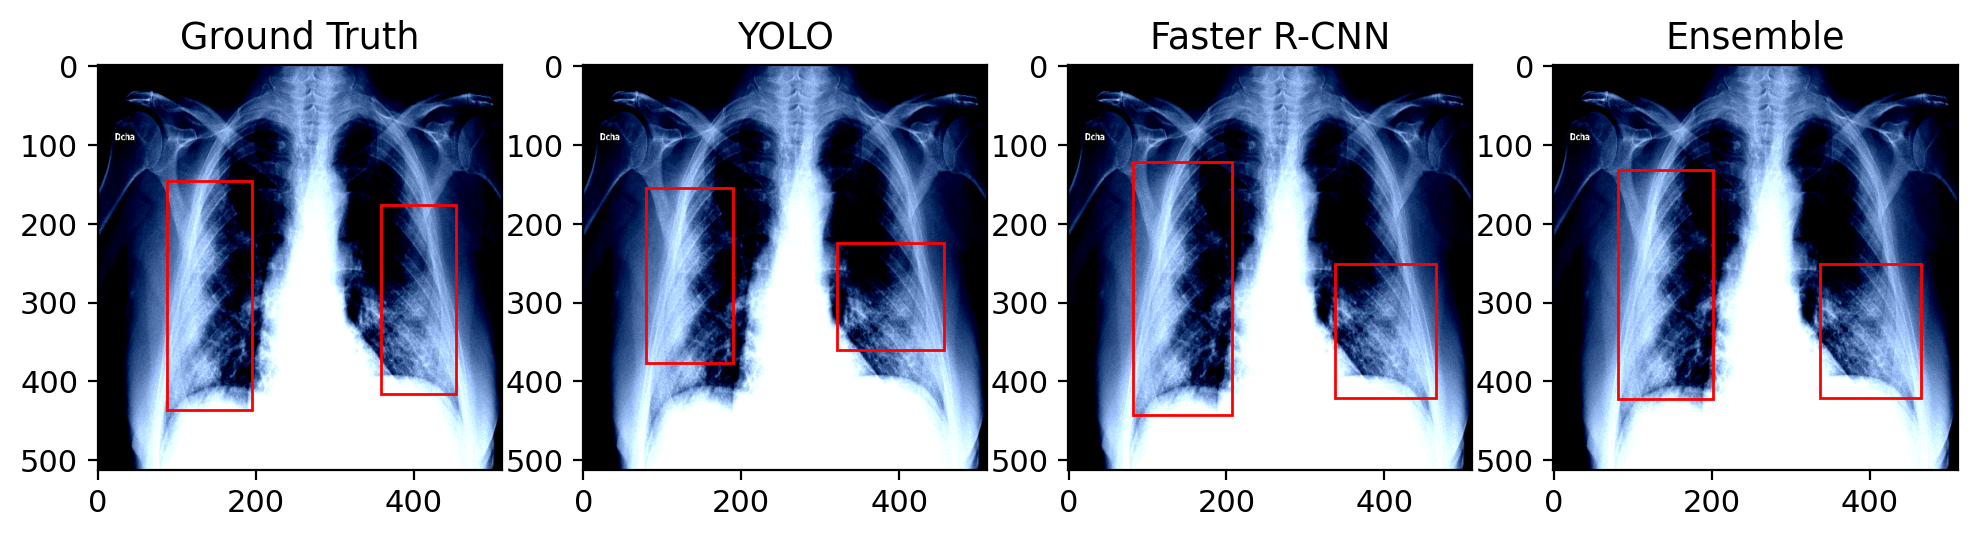
\includegraphics[width=0.6\linewidth]{img/combo.png}
	\caption{Prediction Results on a random examples from the held-out set.}
	\label{fig:combo_eval}
\end{figure*}

To show also a qualitative comparison, figure \ref{fig:combo_eval} shows five different samples from the held-out set and their corresponding predictions of the Faster \ac{R-CNN}, \ac{YOLO} and Ensemble model. It can be observed that both the models already detect affected regions very well, especially in terms of absolute position and agree in most of the predictions, but also struggle in finding the perfect magnitudes of the boxes. Further, the results reveal also some problems of the models as visualized in the third and fifth example, where both models and ultimately the ensemble fails to detect rather small bounding boxes. In addition, the \ac{YOLO} predicts smaller boxes relative to the Faster \ac{R-CNN} in most cases leading to final results that are mainly driven by the latter predictions despite us designing the weights such that both models should contribute equally which is shown in the fifth example of figure \ref{fig:combo_eval}. 

To conclude this section, we showed that both models perform well on the task of detecting COVID-19 affected regions on chest X-rays, reaching the best results by combining a \ac{YOLO} and Faster \ac{R-CNN} model by a confidence score dependent bounding box fusion, but still leaving some open room for improvements (as will be discussed in chapter \ref{chapter:conclusion}).

\section{Evaluation of Study-Level Model}
\sectionauthor{Written by Torben Krieger}
The training of the image classification model was not straight forward and even after various optimizations the validation loss fluctuated. Figure \ref{fig:study-validation-metrics} shows Accuracy, Precision, Recall and F1 score for the performed validations during training. Although all metrics are increasing over the training time, the slope of the increase is small. The total difference between the starting values and the metrics after 58 epochs is limited. The Precision metric shows most fluctuations, one of the highest values was already reached within the second epoch. Only within the last quarter of the training the fluctuation seems to be lower. One reason for less fluctuation at the end of the training could be the used \textit{Cosine Annealing}, therefore the smaller learning rate prevents to big updates.
\begin{figure*}
	\centering
	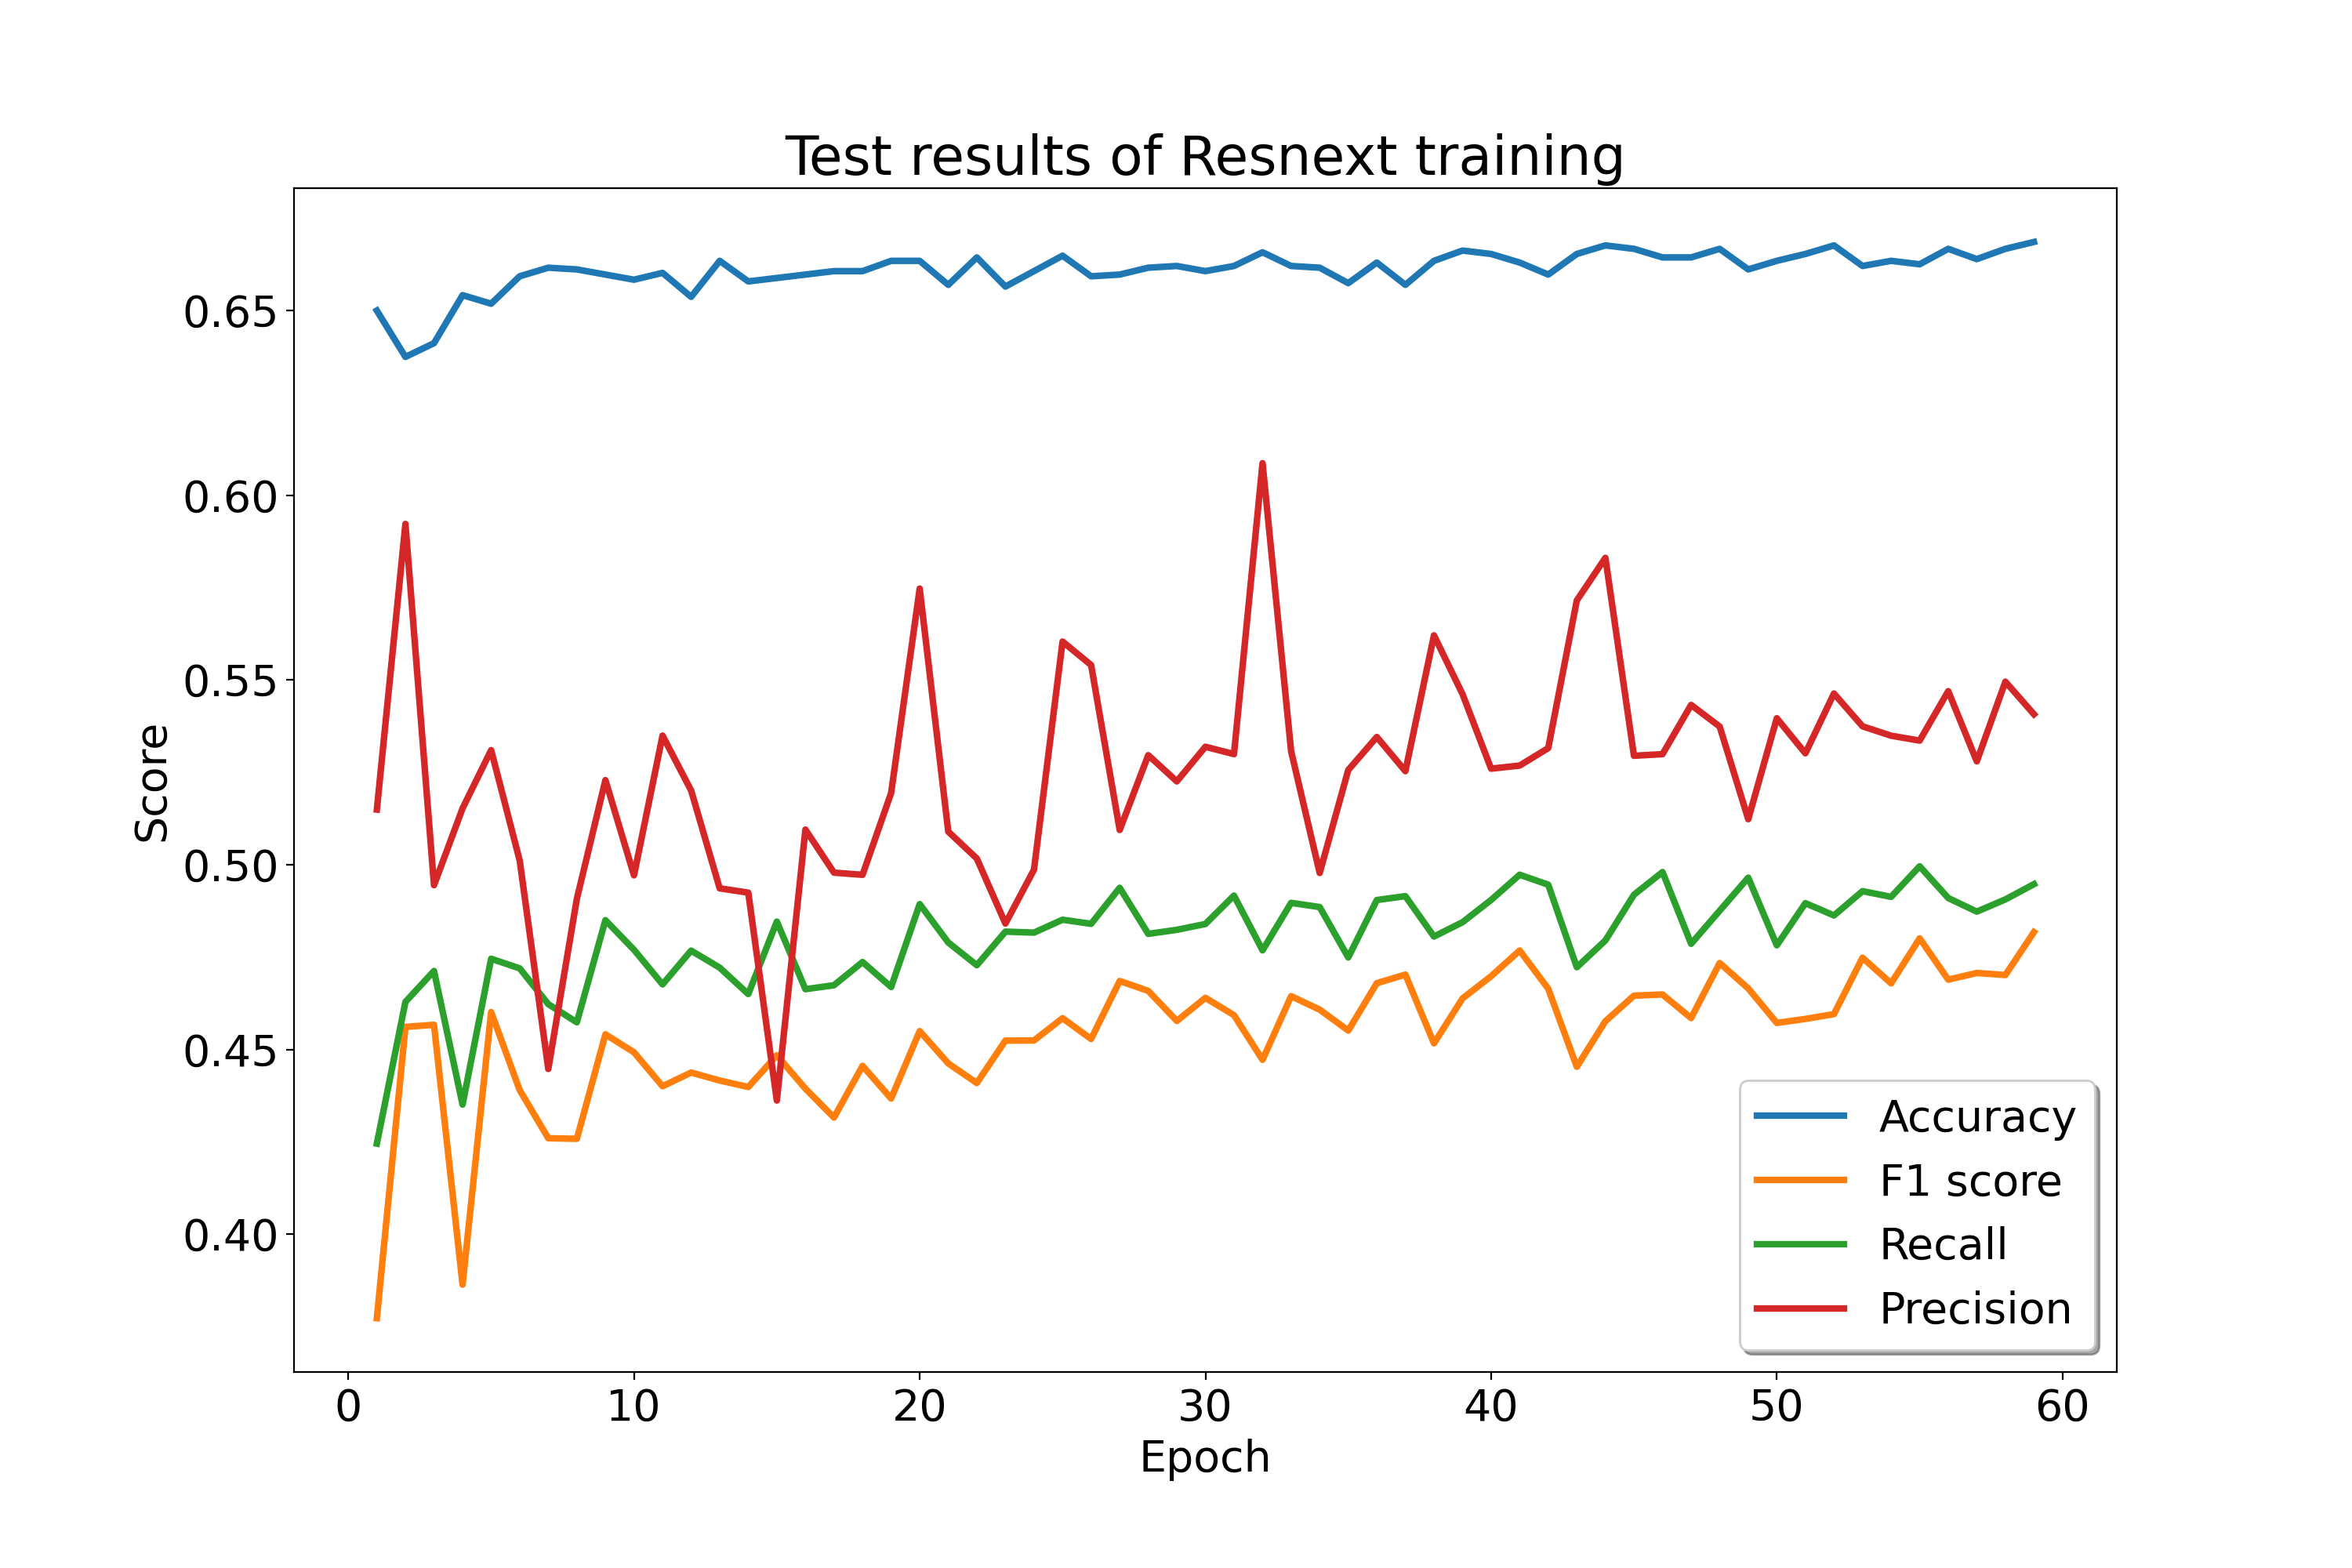
\includegraphics[width=.7\linewidth]{img/test_metrics_study_58.png}
	\caption{Validation metrics of the classification model during training.}
	\label{fig:study-validation-metrics}
\end{figure*}

After the training a test of the image classification model was executed using a test set. The final metrics for that test could be found in table \ref{table:study-results}. Although the metrics are better as the results for the initial pre-training on the NIH dataset we have to stress here that the classification was done for four classes only. The metrics include also the \ac{mAP} which is quite uncommon for classification tasks. Reasons to include it here is that the submissions of the Kaggle Challenge are rated using \ac{mAP}@50 for both, the detection and classification task, in a combined fashion. The formal submission file has to provide a pre-defined dummy bounding box for each study-level classification. The \ac{IoU} threshold of 50\% is therefore irrelevant for the study task and the metric simplifies to simple \ac{mAP}. The calculation of the \ac{mAP} value for our test allows us to compare our results with competitors of the challenge without doing a formal submission. As reference, the first place of the challenge reported a \ac{mAP} of 0.598 for the classification task only \autocite{SIIMFirstPlace}. However they are using an ensemble of models with greater input sizes and performed pre-training on several other datasets as well as specifically for detection of normal pneumonia first. Still it has to be noted that the \ac{mAP} values reported by the competitors were calculated on the hidden held-out dataset of the challenge.
\begin{table}
	\begin{tabular}{l|l}
		&    Study-Level Model  \\ \hline
		Accuracy 		& \textbf{0.669} \\
		mean Recall		& \textbf{0.495} \\
		mean Precision	& \textbf{0.541} \\
		F1-score		& \textbf{0.482} \\
		mAP 	    	& \textbf{0.405} \\
	\end{tabular}
	\centering
	\caption{Test metrics for the image classification model.}
	\label{table:study-results}
\end{table}
Figure \ref{fig:study-confusion-matrix} contains the confusion matrix for the test run. It is observable that our model classifies most images as \textit{Typical}. Besides this the class \textit{Negative} is classified often. The two remaining classes \textit{Indeterminate} or \textit{Atypical} are predicted seldom. By comparing with section \ref{data:siim} it is detectable that this roughly maps to the imbalance of the SIIM dataset. Thus over sampling the dataset or weighting of the loss function for underrepresented classes would be the next attempts to improve the classification. However we did not had the time to test these approaches. Apart from this the confusion matrix indicates that most images of the classes \textit{Typical} and \textit{Negative} were predicted correctly.
\begin{figure*}
	\centering
	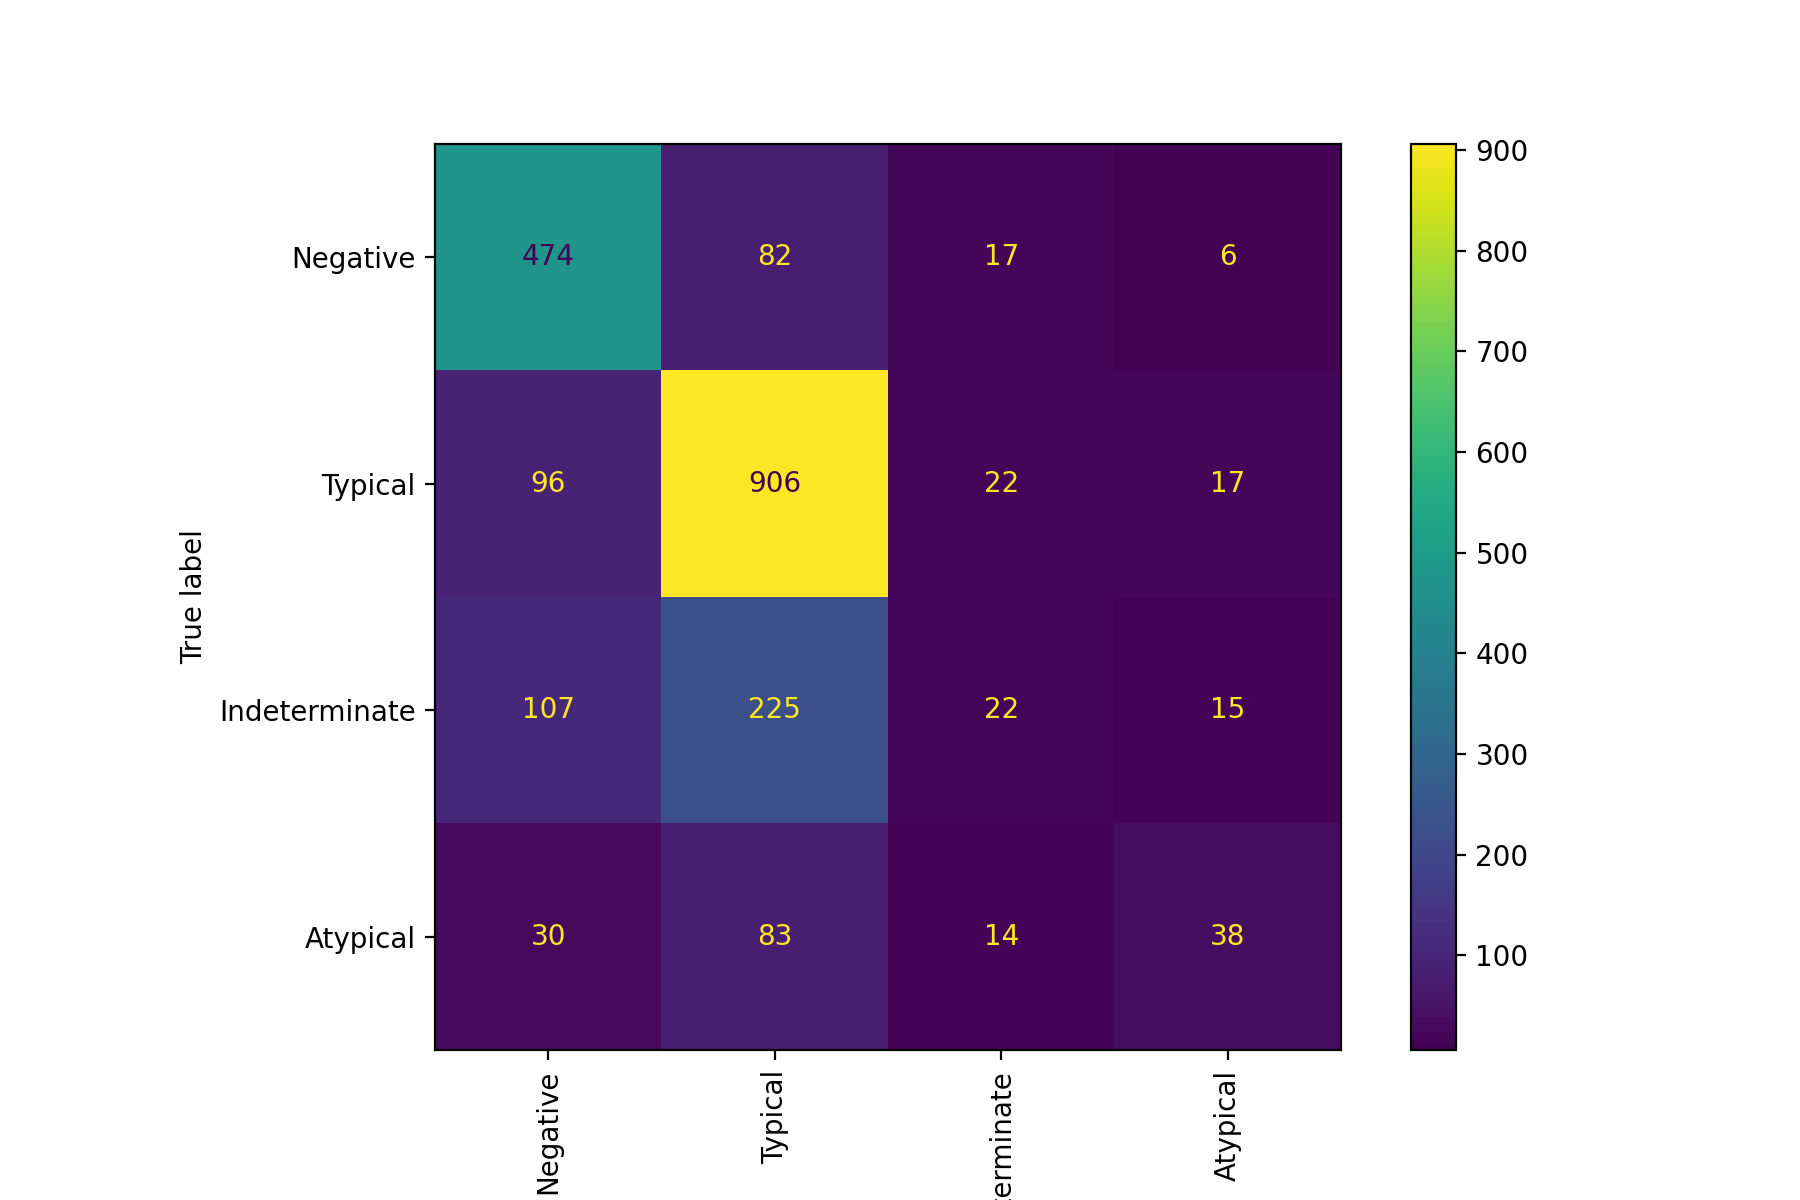
\includegraphics[width=.7\linewidth]{img/confusion_study_58.png}
	\caption{Confusion matrix for the image level classification.}
	\label{fig:study-confusion-matrix}
\end{figure*}
Closing this section we have to conclude that our image classification model not meets the expectations we had. However at least for the two most important classes out of the four classes a acceptable classification performance is observable. Which means that our model is at least somehow able to tackle the underlying problem to detect COVID-19. Possible improvements or alternatives will be discussed in chapter \ref{chapter:conclusion}.
